% !TEX root = ../main.tex
\section{Preliminary Analysis}
\label{sec:preliminary}
In this section, we present the basic ideas and the preliminary results of our attacks.


\begin{figure*}[htbp]
	\centering
%	\subfigure[Original RGB image]{
%		\includegraphics[width=0.23\textwidth]{figures/preanalysis_rgb_1.png} 
%	}
	\subfigure[Printed RGB photo]{
		\includegraphics[width=0.28\textwidth]{figures/preanalysis_rgb_2.png} 
	}
	\subfigure[Digital adversarial example]{
		\includegraphics[width=0.28\textwidth]{figures/preanalysis_rgb_3.png} 
	}
	\subfigure[Printed adversarial photo]{
		\includegraphics[width=0.28\textwidth]{figures/preanalysis_rgb_4.png} 
	}
\vspace{-0.15in}
	\caption{Spoofing RGB-based liveness detection with adversarial photos. (a) Printed photo of a legitimate user with a RGB confidence score: 0.06, (b) Digital adversarial example with a RGB confidence score: 0.96, and (c) Printed adversarial photo with a RGB confidence score: 0.34. }
	\label{preanalysis_rgb}
	\vspace{-0.15in}
\end{figure*}

\begin{figure*}[pt]
	\centering
			\subfigure[Original RGB image]{
			\includegraphics[width=0.28\textwidth]{figures/color1115200905_1.png} 
		}
		\subfigure[Original depth image]{
			\includegraphics[width=0.28\textwidth]{figures/preanalysis_depth_1.png} 
		}
		\subfigure[Replayed depth image]{
			\includegraphics[width=0.28\textwidth]{./figures/preanalysis_depth_2.png} 
		}
%	\subfigure[Replayed depth image with noise reduction]{
%		\includegraphics[width=0.23\textwidth]{./figures/preanalysis_depth_3.png} 
%		}
	\vspace{-0.15in}
		\caption{Spoofing depth-based liveness detection by replaying structured-light patterns. (a)  Original RGB and (b) depth images with a RGB-D confidence score: 0.99, and (c) Replayed depth image with a RGB-D confidence score: 0.02. }
			\vspace{-0.15in}
		\label{preanalysis_depth}
%	\begin{minipage}[t]{0.5\textwidth}
%		\subfigure[Original infrared image]{
%			\includegraphics[width=0.46\textwidth]{figures/preanalysis_ir_1.png} 
%		}
%		\subfigure[Replayed infrared image]{
%			\includegraphics[width=0.46\textwidth]{figures/preanalysis_ir_2.png} 
%		}
%		\caption{The infrared image replay for IR modality. (a) the original infrared image of legitimate user with liveness confidence score : 0.99; (b) the infrared image replayed through infrared projector with livness confidence score : 0.99.}
%		\label{preanalysis_ir}
%	\end{minipage}
\end{figure*}

\subsection{Basic Idea}
In this paper, we investigate the feasibility of spoofing face authentication with a printed photo by bypassing its 3D liveness detection.
Since 3D liveness detection utilizes both the RGB and depth information for detection, we shall bypass its RGB and depth detection models simultaneously.  

For the RGB-based liveness detection model, it can detect photos by analyzing their edges, textures, and moire patterns in normal circumstances. However, since those models are usually based on deep learning algorithms, they have the possibility of being vulnerable to adversarial attacks. Thus, a naive trial is to utilize printed adversarial photos to bypass it. 


For the depth-based liveness detection model, it calculates the depth information by measuring the displacement of the reflected scatter pattern and the original scatter pattern, and uses the special geometric structure of the human face to determine whether the face image is from a real human face.
However, the infrared camera only captures infrared images and does not identify the source of the scatter patterns. As a result,  we may create forged depth information by projecting artificial scatter patterns. 



In the following, we present the preliminary results of the aforementioned ideas.
\subsection{Preliminary Results }

\textbf{Spoofing RGB-based Liveness Detection.} \texttt{DepthFake} utilizes adversarial noises on photos to spoof against the RGB-based liveness detection.
To investigate, we conducted a feasibility test by generating adversarial examples against the RGB module of a commercial liveness detection SDK, i.e., the Baidu Cloud SDK. Specifically, we first captured an RGB image of a legitimate user and  printed it out as a spoofed photo, then we used a black-box adversarial attack method called SimBA \cite{guo2019simple} to generate an adversarial example in the digital world, and finally printed it out as the adversarial photo to investigate whether it can bypass the liveness detection in the real world. 

From the results in Fig.~\ref{preanalysis_rgb}, we find that the RGB-based liveness detection model of the Baidu Cloud SDK does suffer from adversarial attacks. An adversarial example in the digital world can bypass the RGB-based liveness detection with a score of 0.96. Although its attack effectiveness decreases after being printed, it can still get a score of 0.34, higher than that of a printed photo without adversarial perturbations (0.06). 

By comparing the adversarial example in the digital world (Fig.~\ref{preanalysis_rgb} b) and the printed adversarial photo in the real world (Fig.~\ref{preanalysis_rgb} c), we find that the color distortion caused by the printing-capturing process impairs the attack effectiveness. As a result, to guarantee an effective photo attack in the real world, simply generating an adversarial example is not enough. More work shall be done on improving its robustness in the real world by reducing the impacts from color distortions caused by printing and capturing.


\begin{figure*}[pt]
	\centerline{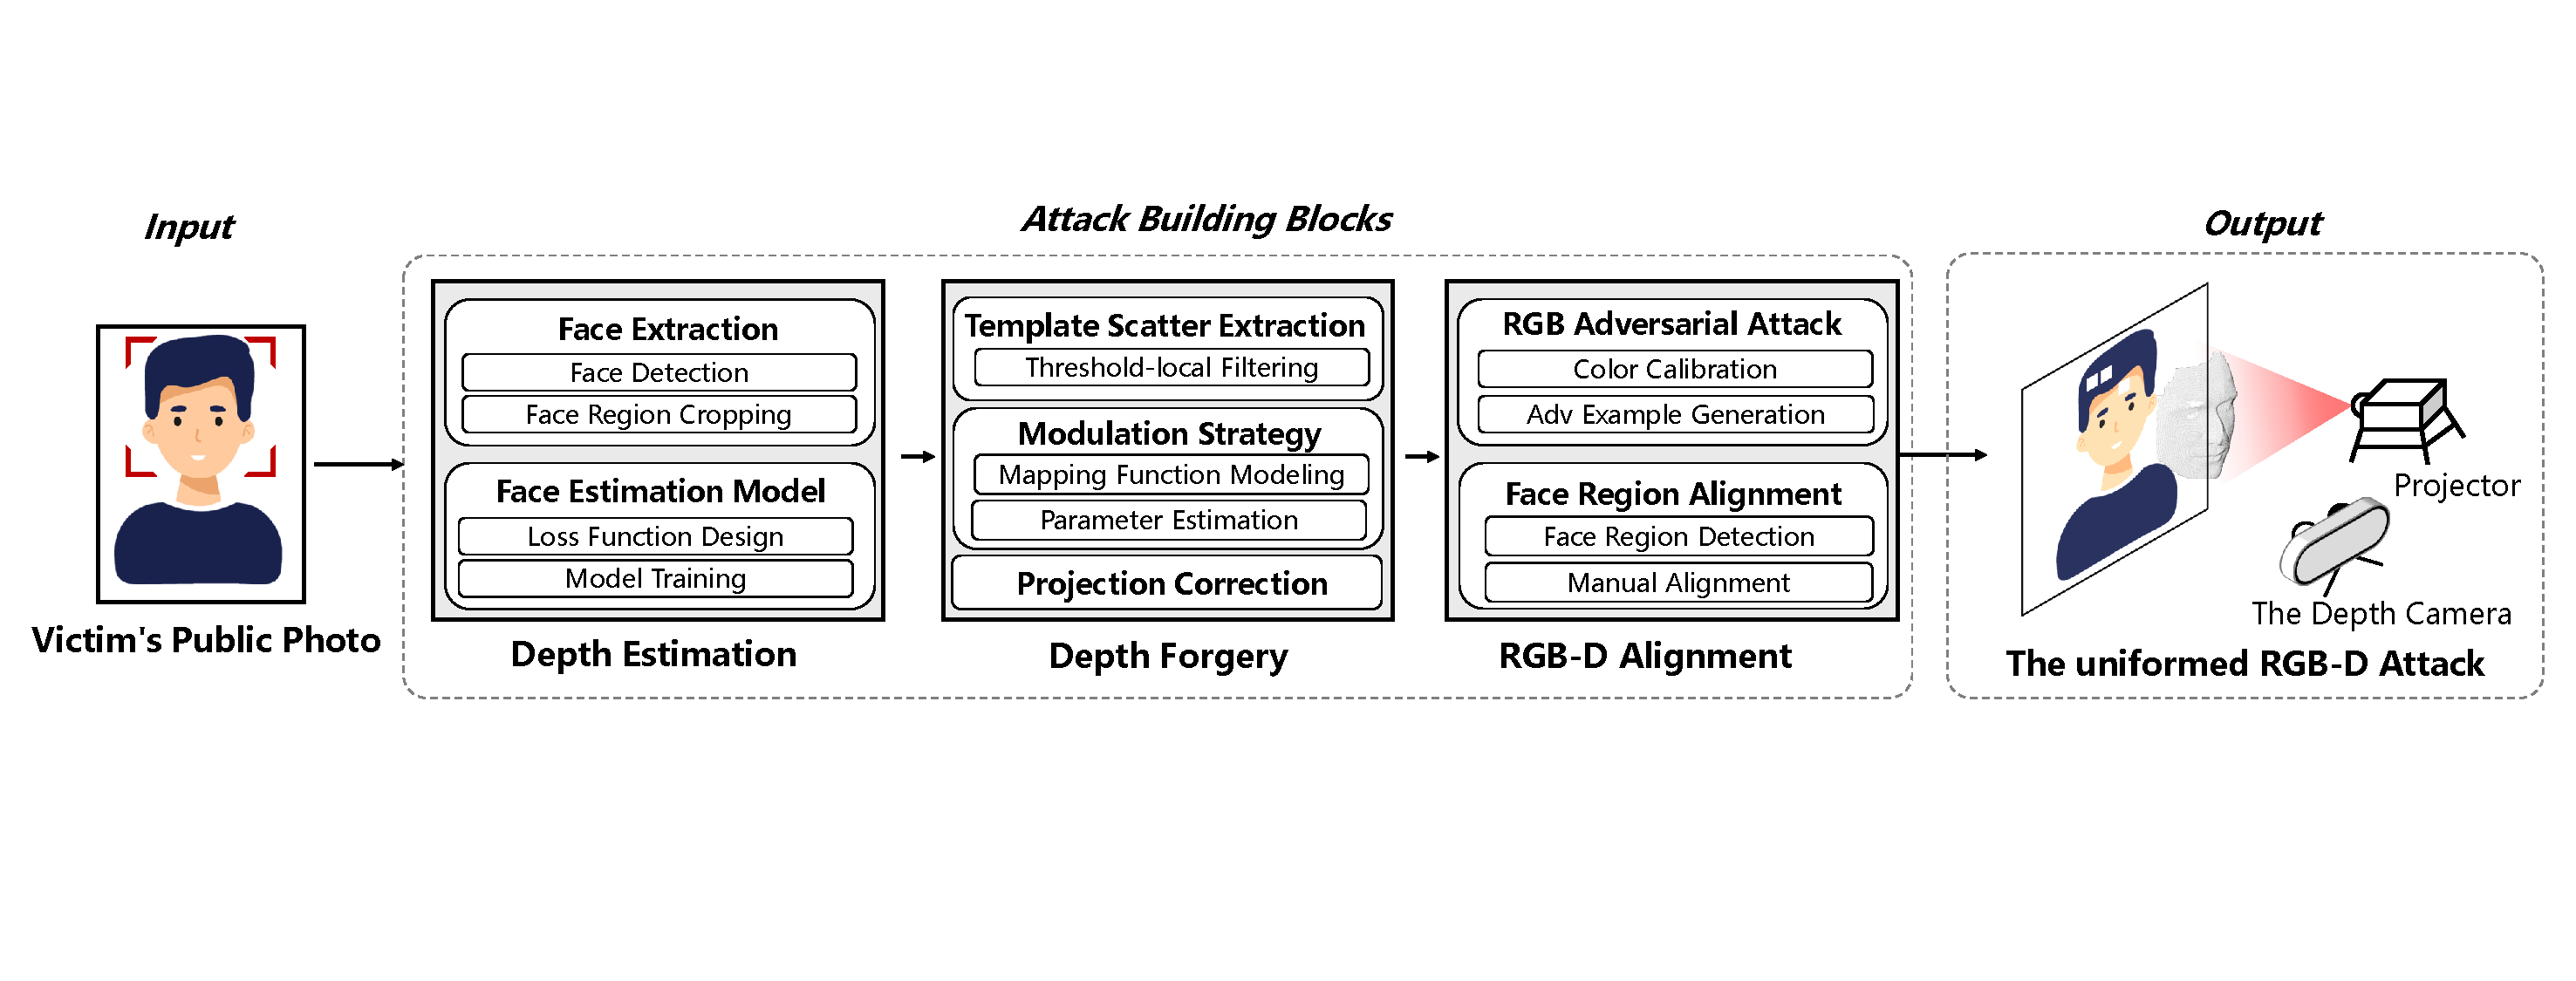
\includegraphics[width = \textwidth]{figures/overview_1.png}}
	\vspace{-0.15in}
	\caption{Overview of \texttt{DepthFake} attack: The adversary first captures a legitimate user's face information with a 3D camera. Then, she uses the face information to generate an adversarial photo and a structured-light scatter pattern projected through an infrared projector to spoof the 3D liveness detection and thus the face authentication system. }
	\label{overview}
		\vspace{-0.15in}
\end{figure*}

\textbf{Spoofing Depth-based Liveness Detection.} \texttt{DepthFake} replays the structured-light patterns to spoof against depth-based liveness detection.
To investigate this idea, we used a structured-light 3D camera Orbbec Astra Pro~\cite{da2020comparison} to capture the infrared scatter pattern reflected by a legitimate user. 
Then, we covered the scatter projector of the structured-light depth camera and used an external infrared projector DLP4500SL02 Evaluation Module~\cite{chong2017intraoperative} to replay the captured scatter pattern to forge the depth information.
The results shown in Fig.~\ref{preanalysis_depth} demonstrate that with the replayed depth image, the confidence score of 3D liveness detection (RGB-D) drops from 0.99 to 0.02.  The reason is that the replayed scatter pattern cannot form the depth of a human face directly since it suffers from noises from background objects during recording. 
%To address it, we perform Histogram Equalization~\cite{abdullah2007dynamic} to reduce the noises in the recorded scatter pattern, which can increase the confidence score from 0.02 to 0.25.

Therefore, simply replaying a structured-light scatter pattern recorded from a  legitimate user can generate the depth information but is not sufficient to forge a human face. More work shall be done on noise reduction to guarantee an effective attack in the real world.

%\textbf{Infrared image replay for IR modality.} The IR-based liveness detection systems use the different reflection features between different materials to identify the non-living objects. The simplest idea is that if we can use infrared projector to simulate the reflection features of human face, we can successfully spoof the IR-based liveness detection systems. To verify its feasibility, we firstly capture the infrared image of human face, and then replay it to a reflector plate. Finally, we used the Baidu Cloud SDK to perform liveness detection on the replayed infrared image. 

%The result is shown in Figure.~\ref{preanalysis_ir}, we observe that the replayed infrared images can get the same high confidence score as the original infrared image. It proves that the replayed infrared image can simulate the reflection features of real face and successfully spoof the IR-based liveness detection system.
